\section{Proyecto principal}
%
%
Este trabajo trataba de la optimización del gasto energético de una empresa que contaba con hornos de fundición. Para ello, se tuvieron que realizar predicciones del precio de la electricidad mediante modelos estadísticos. Posteriormente, se modelizó el proceso de fundición llevado a cabo en la fábrica y por último se trató de optimizar la selección de los materiales a fundir, dependiendo del espacio disponible en fábrica y el precio de la luz en cada tramo horario, estimado previamente.
%
%
\subsection{Predicción de precios de la luz}
%
%
%
%
Para llevar a cabo un modelo predictivo de de los precios de la luz para una empresa hemos de realizar una serie de pasos. En primer lugar, como es evidente, debemos conocer y entender qué es lo que queremos predecir, bajo qué condiciones y qué variables afectan al precio de la luz, tanto naturales, como puede ser la demanda, la generación de ciertos tipos de energía, como aquellas relacionadas con la legislación vigente. Posteriormente debemos decidir cómo se extraeran los datos necesarios. Puesto que estamos hablando de un proyecto real, la empresa espera un proceso automatizado por lo que se debe tener en cuenta una extracción periódica de datos.

Una vez planteado el contexto en el que vamos a movernos, debemos decidir qué modelos probar, conociendo sus ventajas y desventajas. Mi elección, basada en búsquedas de desarrollos similares, fue optar por tres modelos:
\begin{description}
    \item[SARIMAX] Modelo estadístico clásico
    \item[XGBoost] Modelo de \textit{machine learning}
    \item[TFT] Modelo de \textit{deep learning}
\end{description}

Por último, por requisitos del proyecto, la predicción se realizaba a un mes vista, lo cual como es lógico, no es óptimo. Sin embargo, esto era algo fijo por lo que los resultados esperados son mejorables, recortando el horizonte de predicción y reentrenado los modelos con mayor asiduidad.
%
%
%
\subsubsection{Estudio y comprensión del mercado}
%
%
%
Dado que la empresa es una electrointensiva no se rige por el régimen general del pequeño consumidor (PVPC). Para la toma de datos de la variable objetivo, el precio de la luz, se consultó el precio del mercado SPOT diario, que es el que regula la venta de luz al por mayor.

Para calcular exactamente, dentro de lo que podemos entender como \textit{exacto} en un modelo de predicción, el precio de la luz debemos tener en cuenta tanto el precio de venta como los peajes. Estos últimos son valor añadido a la factura de la luz que depende del tipo de empresa y de la hora de consumo. De cualquier forma, en lo que a nuestro modelo se refiere, únicamente nos interesa el preio del mercado SPOT diario, que viene dado de manera horaria.
%
%
%
\subsubsection{Obtención y preparación de los datos}
%
%
%
Los datos se obtuvieron a través de la API pública proporcionada por ESIOS (Sistema de Información del Operador del Sistema Eléctrico), que permite acceder a los precios horarios históricos, así como a otros indicadores del sistema eléctrico. De manera adicional al precio de la luz, y como se ha comentado previamente, se tomaron variables explicativas, es decir, que se cree que tienen relación y afectan al precio de la que queremos. En este caso, se tomó: La demanda real de consumo, la generación de energía eólica y solar.

En lo relativo a la preparación de los datos, salvando las diferencias en función de la implementación del modelo, el procedimiento fue similar: Una vez descargados los datos se formatean de manera que tengamos aquellos valores que queremos, es decir, el precio, demanda, etc. y la fecha en la que se dio. Además, de cara a refinar nuestro modelo, se introdujeron variables temporales como el día de la semana, día del mes o mes del año. Un estudio mucho más exaustivo puede hacerse incluyendo más variables o con más combinaciones. En \cite{TFG_prediccion} puede verse como incluyen el precio del gas o la emisión de CO$_2$ entre otro, llevándoles a mejores resultados, aunque con mayor trabajo.
%
%
%
\subsubsection{Análisis exploratorio}
%
%
%
Este proceso consiste en la observación de los datos, su representación en diferentes formas con el fin de decidir características del modelo. El estudio consistió en graficar respecto del tiempo el histórico de datos, implementar una matriz de correlación para observar las relaciones entre las distintas variables y boxplot para estudiar el comportamiento de nuestra serie. En las siguientes figuras podemos visualizarlo:
\begin{figure}[H]
\centering
\begin{subfigure}[b]{0.35\textwidth}
\centering
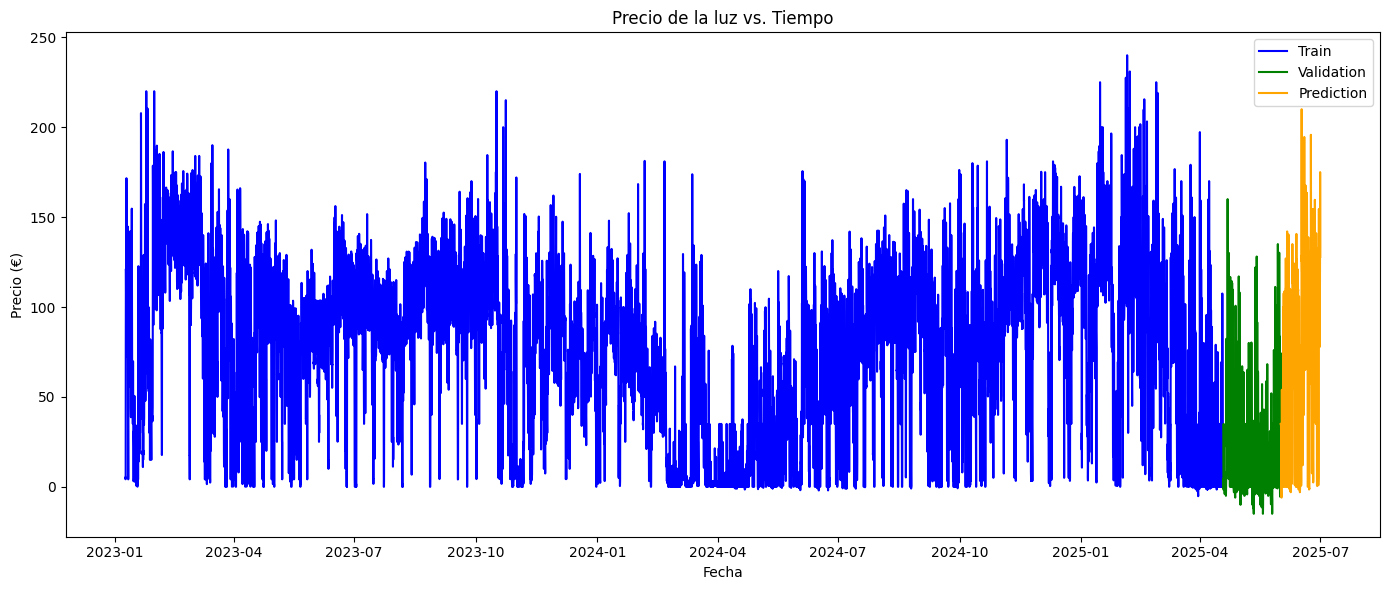
\includegraphics[width=\textwidth]{figuras/historico_precios.png}
\caption[Precio de la luz respecto del tiempo]{.}
\label{Precio vs tiempo}
\end{subfigure}
\begin{subfigure}[b]{0.35\textwidth}
\centering
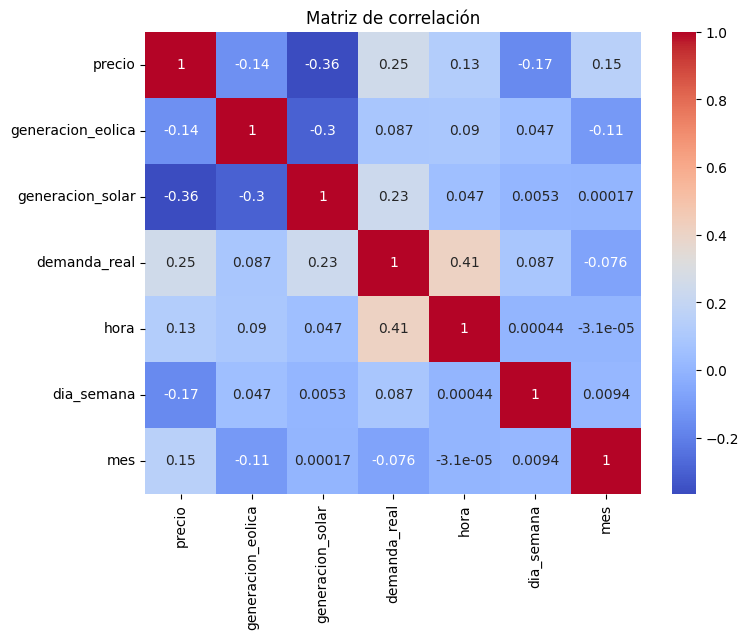
\includegraphics[width=\textwidth]{figuras/matriz_correlacion.png}
\caption[Matriz de correlación]{.}
\label{Matriz de correlacion}
\end{subfigure}
\begin{subfigure}[b]{0.35\textwidth}
\centering
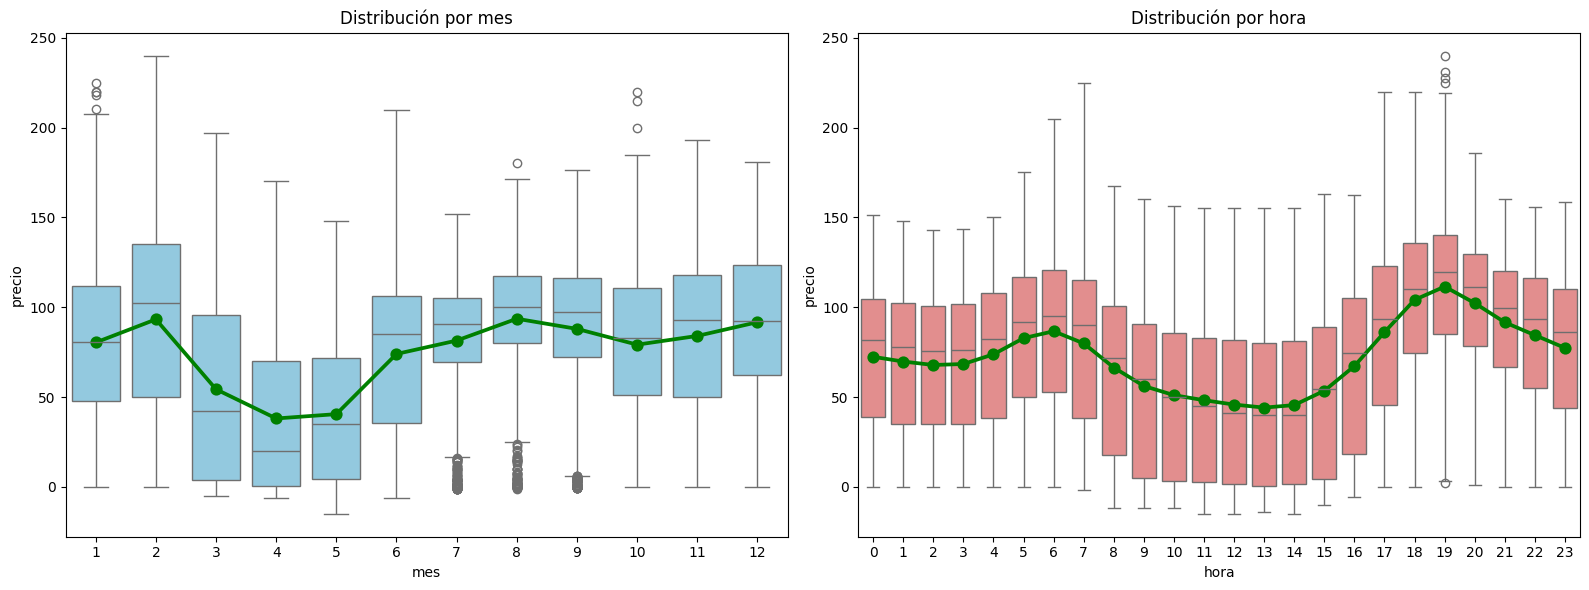
\includegraphics[width=\textwidth]{figuras/boxplots_precios.png}
\caption[Boxplot diario]{.}
\label{Booxplotdiario}
\end{subfigure}
\begin{subfigure}[b]{0.35\textwidth}
\centering
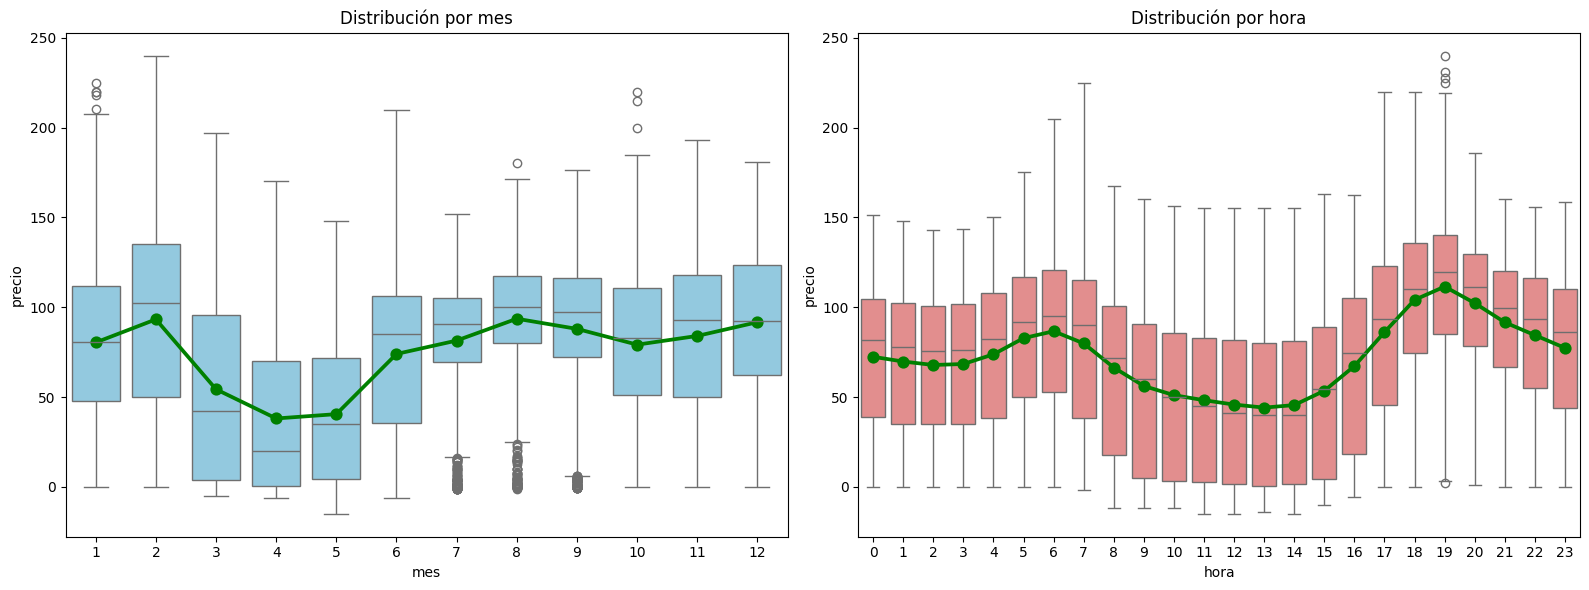
\includegraphics[width=\textwidth]{figuras/boxplots_precios.png}
\caption[Boxplot anual]{.}
\label{Boxplotanual}
\end{subfigure}
\caption{Figuras del análisis exploratorio.}
\label{Análisis exploratorio}
\end{figure}
A partir de estos datos, como se puede observar en la figura \Cref{Precio vs tiempo}, se divide el histórico de datos en un conjunto de entrenamiento, otro de test y se deja uno de validación, en este caso de un mes, al igual que la predicción que queremos realizar, para comprobar el funcionamiento \textit{real} de nuestro modelo \footnote{Este proceso se utilizó tanto en la SARIMAX como en el XGBoost, como se explicará más adelante, el TFT no requiere un \textit{train} y \textit{test} setm, le indicas por configuración el número de pasos que tomas del histórico y el número de ellos para la predicción.}

Observando la matriz de correlación puede verse también que la variable más significativa es BLA, si bien es cierto que todas se encuentran en un mismo rango de relación. En último lugar, de los boxplot podemos observar como los meses de abril y mayo son los de menor precio mientras que los de noviembre y diciembre el precio aumenta significativamente. Del mismo modo, en el ámbito diario podemos observar como las denominadas \textit{horas valle} se corresponden con el tramo de 8-10 y las \textit{horas pico} con 13-17.
%
%
%
\subsubsection{SARIMAX}
%
%
%
Este es un modelo estadístico clásico para la predicción de series temporales. Su fortaleza radica en su capacidad para modelar explícitamente tres componentes clave de la serie:

\begin{itemize}
    \item \textbf{Tendencia (I - Integrado):} Se logra a través de la diferenciación para hacer que la serie sea estacionaria.
    \item \textbf{Estacionalidad (S - Seasonal):} Captura patrones que se repiten en intervalos fijos (por ejemplo, diarios o semanales).
    \item \textbf{Variables (X):} Permite incluir predictores externos, como la demanda o la generación de energía.
\end{itemize}

El proceso consiste en:
\begin{itemize}
    \item \textbf{Identificación:} El modelo SARIMAX viene caracterizado por los valores $(p,d,q)x(P,D,Q,s)$ donde:
        \begin{itemize}
        \item[$p:$] Orden del componente autorregresivo (AR) no estacional. Indica el número de rezagos de la variable endógena que se incluyen en el modelo.
        \item[$d:$] Orden de diferenciación no estacional. Representa la cantidad de veces que se deben diferenciar los datos para hacer la serie estacionaria.
        \item[$q:$] Orden del componente de media móvil (MA) no estacional. Indica el número de rezagos del error del pronóstico que se incluyen en el modelo.
        \item[$P:$] Orden del componente autorregresivo (AR) estacional.
        \item[$D:$] Orden de diferenciación estacional.
        \item[$Q:$] Orden del componente de media móvil (MA) estacional.
        \item[$s:$] Período de estacionalidad, en este caso vemos que $s=24$ de manera natural al tratarse de precios horarios.
    \end{itemize}
    
    \item \textbf{Estimación:} Una vez definidos los órdenes, se ajusta el modelo al conjunto de datos de entrenamiento. El modelo aprende los coeficientes que ponderan la importancia de los valores pasados, los errores de pronóstico pasados y las variables exógenas.
\end{itemize}

La predicción con SARIMAX es un proceso iterativo o recursivo:
\begin{itemize}
    \item \textbf{Entrenamiento:} Al igual que con otros modelos, se reentrena un modelo SARIMAX final con su orden óptimo utilizando todos los datos históricos disponibles para maximizar la información aprendida.
    
    \item \textbf{Predicción:} Para predecir el horizonte futuro (ej. las próximas 24 horas), el modelo:
    \begin{itemize}
        \item Predice el primer paso (t+1) utilizando todos los datos históricos reales.
        \item Para predecir el segundo paso (t+2), utiliza los datos históricos y la predicción que acaba de hacer para t+1 como si fuera un dato real.
    \end{itemize}
\end{itemize}

Este proceso se repite para cada punto en el horizonte de predicción.

En nuestro caso, para determinar los órdenes de los hiperparámetros del modelo, se analizan las funciones de autocorrelación (ACF) y autocorrelación parcial (PACF). La ACF mide la correlación de la serie consigo misma en diferentes rezagos, mientras que la PACF mide esta misma correlación eliminando la influencia de los rezagos intermedios.

En las siguientes imágenes podemos ver los gráficos de ACF y PACF para la serie de precios de la luz, lo que nos permite identificar los patrones de estacionalidad y los órdenes de los modelos.

\begin{figure}[H]
    \centering
    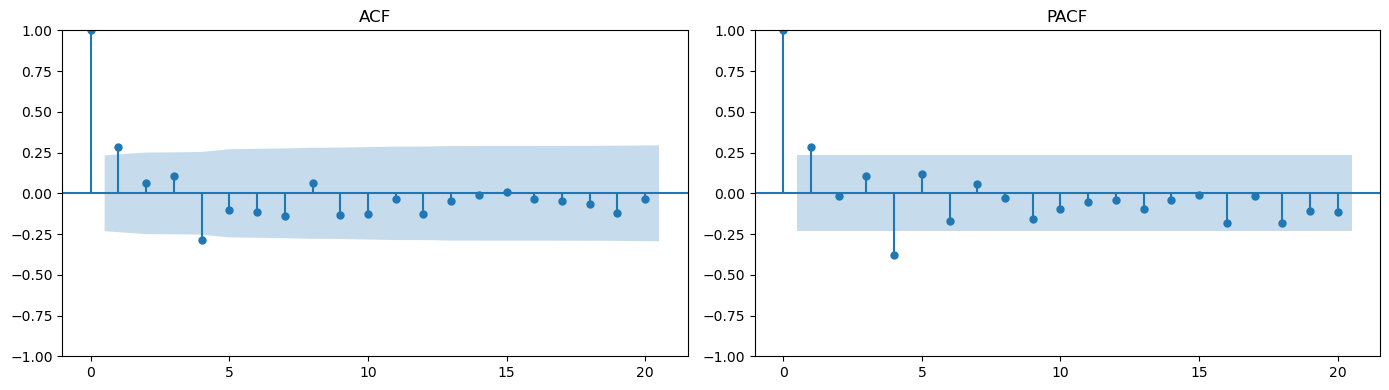
\includegraphics[width=0.7\linewidth]{figuras/ACF_PACF.png}
    \caption[ACF y PACF para d=D=0]{ACF y PACF de la serie de precios de la luz sin diferenciar. Se observa una clara estacionalidad y una autocorrelación que decae lentamente, lo que sugiere la necesidad de diferenciación.}
    \label{fig:ACF_sin_diferenciar}
\end{figure}
\begin{figure}[H]
    \centering
    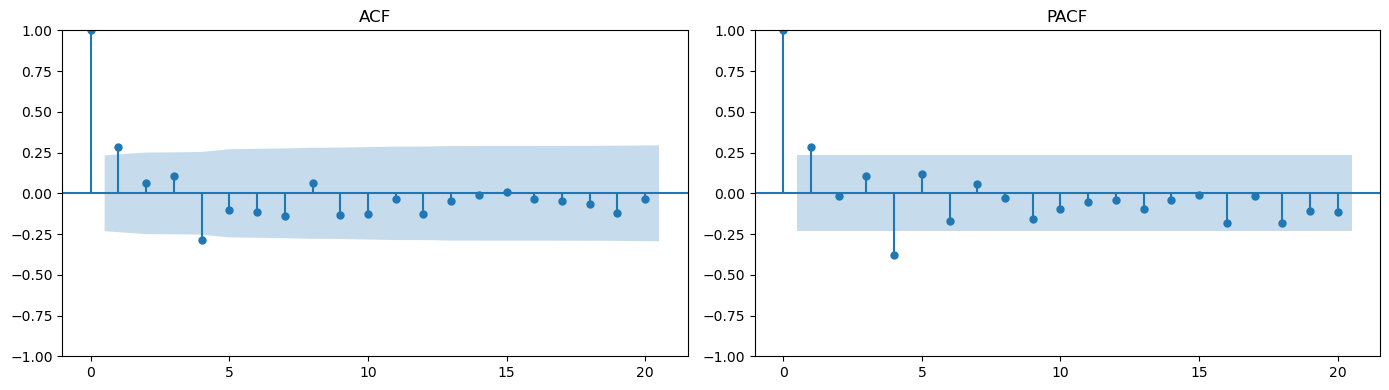
\includegraphics[width=0.7\linewidth]{figuras/ACF_PACF.png}
    \caption[ACF y PACF para D=1, s=24]{ACF y PACF de la serie de precios con diferenciación estacional. Aunque la estacionalidad ha sido eliminada, la autocorrelación no estacional aún persiste.}
    \label{diferenciado}
\end{figure}
\begin{figure}[H]
    \centering
    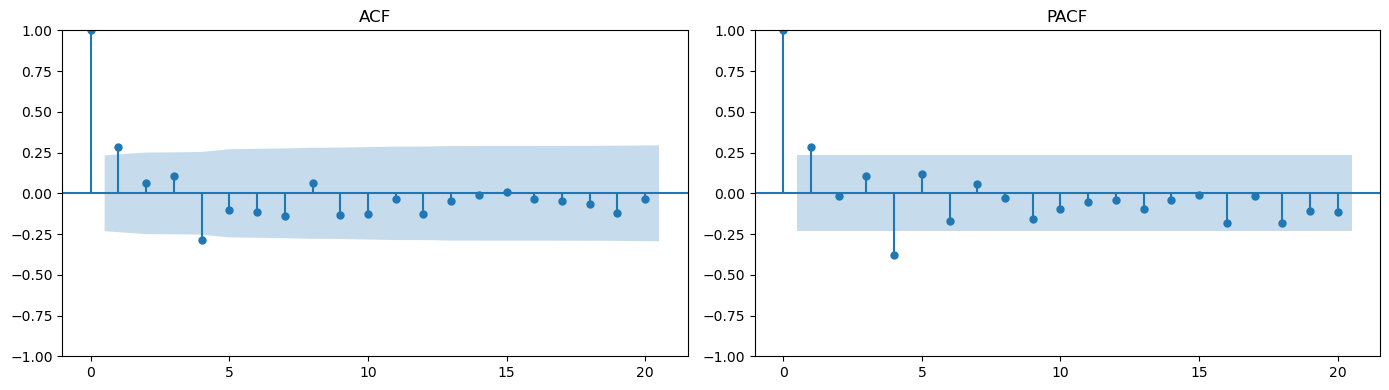
\includegraphics[width=0.7\linewidth]{figuras/ACF_PACF.png}
    \caption[ACF y PACF para d=D=1, s=24]{ACF y PACF de la serie con diferenciación doble. Ahora la serie es estacionaria y los rezagos significativos nos indican los posibles órdenes $p, q, P, Q$.}
    \label{dobledifereniado}
\end{figure}

Basado en el análisis de las funciones de autocorrelación, se han preseleccionado los siguientes tres modelos con sus respectivos órdenes:

\begin{itemize}
    \item \textbf{Modelo 1: SARIMAX(1,1,1)x(1,1,1,24)}:
    Se elige este modelo porque los picos en los gráficos de ACF y PACF de la serie doblemente diferenciada son significativos en el primer rezago no estacional y estacional. Esto sugiere un orden de 1 para los componentes AR, MA, y sus contrapartes estacionales.

    \item \textbf{Modelo 2: SARIMAX(0,1,1)x(0,1,1,24)}:
    Este modelo se considera debido a que, en el gráfico PACF, los picos son más pronunciados en los primeros rezagos, lo que podría indicar la preponderancia de los términos de media móvil.

    \item \textbf{Modelo 3: SARIMAX(2,1,0)x(2,1,0,24)}:
    Se opta por este modelo como alternativa, ya que los gráficos de ACF y PACF también muestran una posible influencia de los segundos rezagos, tanto estacionales como no estacionales.
\end{itemize}

Estos tres modelos serán evaluados y comparados utilizando métricas como el MAE y el RMSE para determinar cuál de ellos ofrece un mejor ajuste a los datos.
%
%
%
\subsubsection{XGBoost}
%
%
%
Este modelo, basado en árboles de decisión, también es relativamente sencillo de implementar aunque, como es habitual en este tipo de modelos, presenta menor interpretabilidad respecto a lo que ocurre dentro del algoritmo. Su robustez radica en la capacidad de aprender patrones complejos mediante un enfoque de ensamblado (\textit{ensemble}) y mejora por aproximación secuencial de errores. Además, se ve reforzado por técnicas de regularización y control del \textit{overfitting}, lo que permite obtener modelos generalizables y eficientes en predicción.Entre las características más destacadas de XGBoost:

\begin{itemize}
    \item \textbf{Regularización integrada:} A diferencia de otros modelos basados en árboles, XGBoost incluye regularización $L_1$ y $L_2$ como parte de la función de coste, permitiendo controlar la complejidad del modelo y reducir el riesgo de \textit{overfitting}
    \item \textbf{Manejo de valores nulos:} Tiene un tratamiento nativo para valores faltantes, aprendiendo automáticamente la mejor dirección en los nodos de decisión.
    \item \textbf{Velocidad y eficiencia:} Permite la construcción de árboles de manera paralela. Además, utiliza una aproximación de segundo orden (Taylor) sobre la función de pérdida, incorporando tanto el gradiente como el hessiano. Esto no solo acelera la convergencia del modelo, sino que también permite trabajar con funciones de pérdida más generales, si bien lo más común es trabajar con el error cuadrático medio.
    \item \textbf{Importancia de variables:} Aunque la interpretabilidad del modelo global es limitada, permite extraer métricas de importancia relativa de cada predictor.
\end{itemize}

El entrenamiento se realiza mediante un enfoque de \textit{boosting}:

\begin{itemize}
    \item \textbf{Inicialización:} Se parte de una predicción base (por ejemplo, la media de la variable a predecir).
    \item \textbf{Aprendizaje secuencial:} Cada árbol posterior intenta corregir los errores residuales cometidos por el conjunto acumulado hasta el momento.
    \item \textbf{Optimización de la función de pérdida:} Se utiliza una aproximación de segundo orden (gradiente y hessiano) para mejorar la precisión de la optimización.
    \item \textbf{Regularización:} Durante el proceso se penaliza la complejidad del modelo (profundidad de los árboles, número de nodos) para evitar \textit{overfitting}.
\end{itemize}
La predicción con XGBoost, al igual que en modelos como SARIMAX, se lleva a cabo de forma secuencial.

Aunque la implementación de este modelo puede parecer más sencilla, es importante comprender las distinas configuraciones que se pueden introducir. La librería \textit{scikit-learn} proporciona herramientas muy útiles para optimizar modelos como XGBoost, en particular \textit{TimeSeriesSplit} y \textit{GridSearchCV}. En el proceso de entrenamiento, nos enfrentamos a dos desafíos principales: la selección de los hiperparámetros óptimos y la evaluación de los errores.

Para la segunda problemática, \textit{TimeSeriesSplit} nos permite dividir nuestro conjunto de entrenamiento en particiones cronológicas, lo que es esencial para las series de tiempo, ya que una división aleatoria rompería la secuencia temporal. De esta manera, podemos obtener múltiples métricas de error (como MAE, RMSE y R$^2$) a lo largo del conjunto de datos y promediarlas para una evaluación más fiable.

Para la elección de los hiperparámetros del modelo, conocida como \textit{hyperparameter tuning}, utilizamos \textit{GridSearchCV}. Esta herramienta prueba sistemáticamente diferentes combinaciones de hiperparámetros dentro de los rangos que le proporcionamos, devolviéndonos la configuración que produce el mejor rendimiento. En esencia, y manera un poco más informal, prueba todas las configuraciones en un rango y nos dice cuál es la mejor en función de uno de los parámetros como puede ser el RMSE.

A continuación, se muestra un fragmento de código que implementa la validación cruzada temporal y la búsqueda de hiperparámetros con \textit{GridSearchCV}.

\begin{lstlisting}[caption={Búsqueda óptima de hiperparámetros y validación cruzada en el modelo XGBoost }, label={TSSyGSXGBoost}]
param_grid = {
    'n_estimators': [300, 325, 350, 375, 400, 425, 450],
    'learning_rate': [0.02, 0.03, 0.04, 0.05, 0.06, 0.07],
    'max_depth': [2, 3, 4, 5]
}

tscv = TimeSeriesSplit(n_splits=5) 

xgb = XGBRegressor(random_state=42, reg_alpha=5, reg_lambda=1)

grid_search = GridSearchCV(
    estimator=xgb,
    param_grid=param_grid,
    scoring='neg_mean_absolute_error',
    cv=tscv,
    n_jobs=-1,
    verbose=2
)
print("------------------------------------")
print("Iniciando búsqueda de hiperparámetros con GridSearchCV...")
print("------------------------------------")
grid_search.fit(X_train, Y_train)
print("<------------ VALORES DE LOS ERRORES ------------>")
print(f"Mejores hiperparámetros encontrados: {grid_search.best_params_}")
print(f"Mejor MAE con validación cruzada: {-grid_search.best_score_:.2f}")
print("------------------------------------")
\end{lstlisting}
print(f"R²: {r2_score(Y_test, Y_test_pred):.4f}")
En el código anterior, los hiperparámetros que se optimizan son \textit{n$\_$estimators}, \textit{learning$\_$rate} y \textit{max$\_$depth}.
\begin{itemize}
    \item \textbf{n$\_$estimators}: Representa el número de árboles de decisión que el modelo construye de forma secuencial. Un mayor número de estimadores puede mejorar la capacidad predictiva del modelo, pero también aumenta el riesgo de \textit{overfitting} y el tiempo de cálculo.
    \item \textbf{learning$\_$rate}: Es un factor de ponderación que controla el peso que tiene cada nuevo árbol de decisión en la predicción final. Un valor más bajo hace que el modelo aprenda de forma más gradual, reduciendo el riesgo de \textit{overfitting}.
    \item \textbf{max$\_$depth}: Limita la profundidad máxima de cada árbol de decisión. Es un hiperparámetro crucial para controlar la complejidad del modelo. Una profundidad más pequeña ayuda a prevenir el \textit{overfitting} al simplificar los árboles.
\end{itemize}
En las siguientes gráficas mostramos los resultados obtenidos en uno de los entrenamientos junto a sus errores:
\begin{figure}[H]
    \centering
    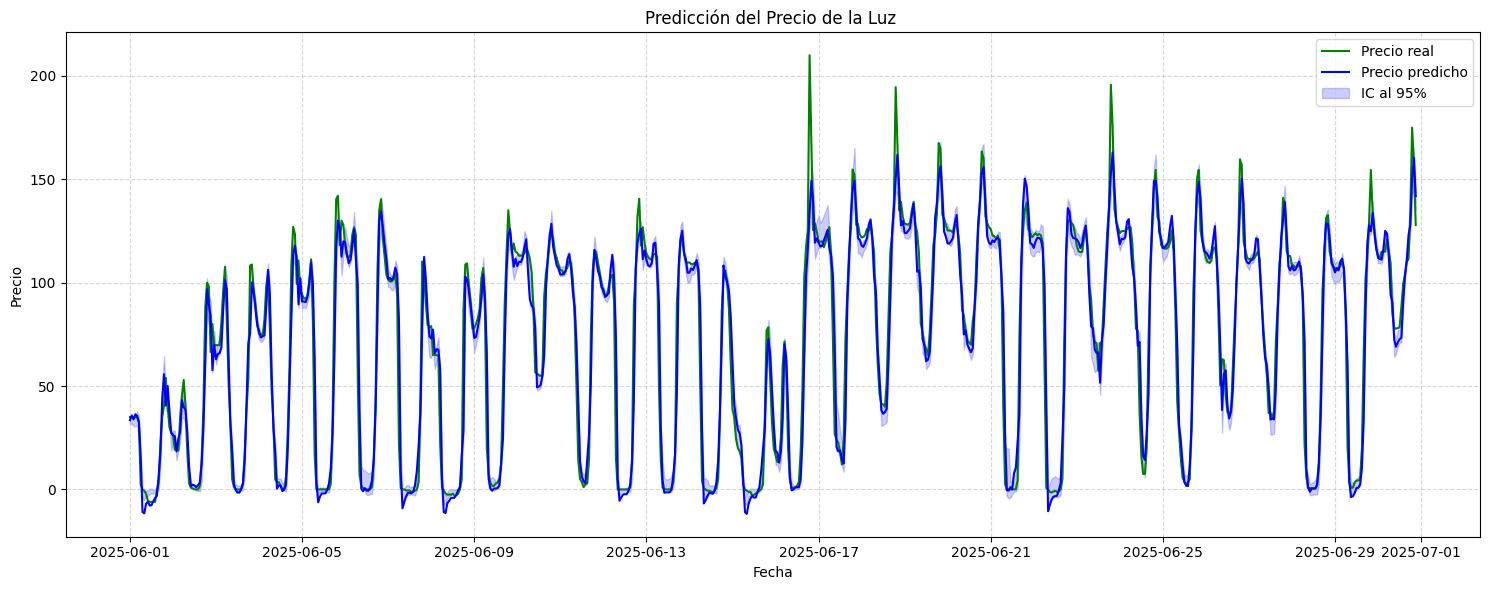
\includegraphics[width=0.7\linewidth]{figuras/XGBoost_prediccion.png}
    \caption[Prediccion con XGBoost]{Se observa una predicción realizada para el mes de junio de 2025 con un entrenamiento del histórico de datos completos.}
    \label{dobledifereniado}
\end{figure}
\begin{figure}[H]
    \centering
    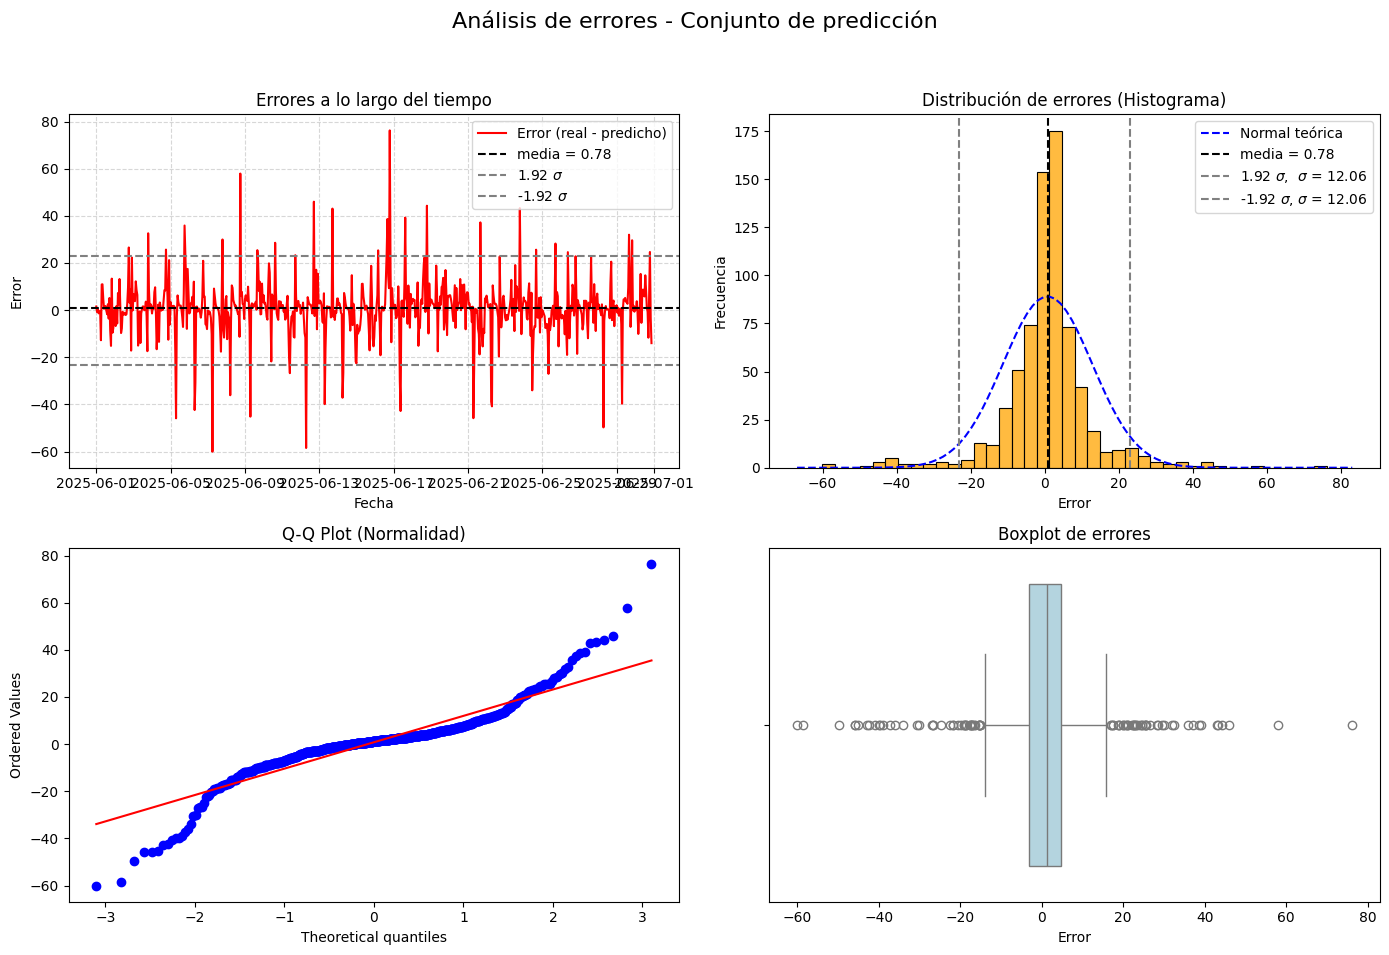
\includegraphics[width=0.7\linewidth]{figuras/XGBoost_errores.png}
    \caption[Errores en prediccion con XGBoost]{Errores del modelo XGBoost, en el que destacan los QQ-plots y el histograma para caracterizar el comportamiento de los mismos. Puede verse en ellos que se distribuyen de forma simétrica, sin colas pesadas aunque no completamente normal.}
    \label{dobledifereniado}
\end{figure}
%
%
%
\subsubsection{TFT}
%
%
%
El Temporal Fusion Transformer (TFT) es una arquitectura de deep learning diseñada específicamente para el forecasting de series temporales multi-horizonte. Combina mecanismos de atención (propios de los Transformers) con redes neuronales recurrentes y capas de gating. Sus características clave son:

\begin{itemize}
    \item \textbf{Manejo de Múltiples Tipos de Variables:} Integra de forma nativa variables estáticas, entradas conocidas en el futuro y variables observadas en el pasado (ej. precio, demanda).
    \item \textbf{Aprendizaje de Patrones a Múltiples Escalas:} Puede identificar patrones temporales tanto a corto como a largo plazo simultáneamente.
\end{itemize}
%
%
%
El entrenamiento consiste en:
%
%
%
\begin{itemize}
    \item \textbf{Preparación de los Datos:} Los datos se estructuran en "ventanas" de entrada de una longitud fija para predecir una "ventana" de salida (ej. las próximas 24 horas).
    \item \textbf{Ajuste del Modelo:} Se entrena una única red neuronal que aprende las interacciones entre todas las variables a lo largo del tiempo.
\end{itemize}
%
%
%
La predicción con TFT se realiza en un solo paso:
%
%
%
\begin{itemize}
    \item \textbf{Reentrenamiento:} Se ajusta el modelo final con todos los datos históricos disponibles.
    \item \textbf{Predicción Multi-Horizonte Directa:} Para generar la predicción, se le proporciona al modelo la última ventana de datos históricos disponibles. En una única pasada hacia adelante (forward pass), el modelo genera directamente todas las predicciones para el horizonte completo.
\end{itemize}
%
%
%
\begin{figure}[H]
    \centering
    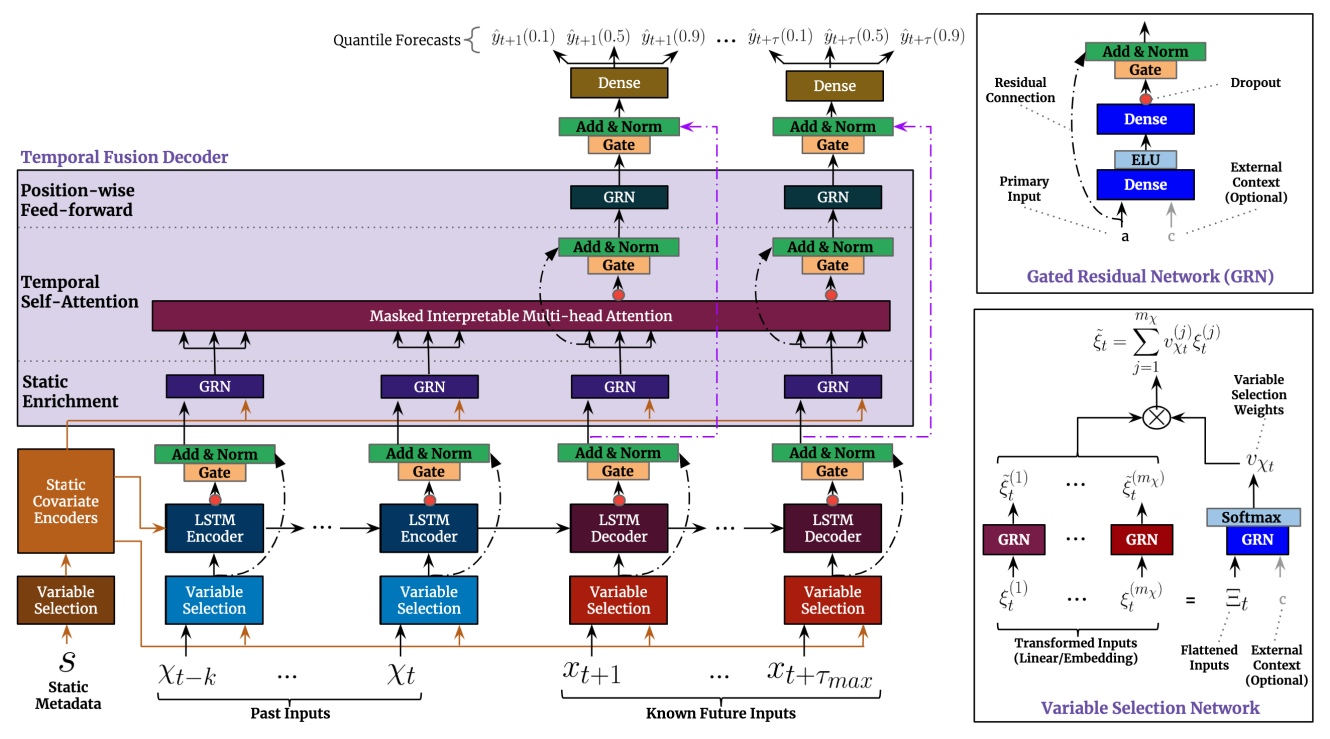
\includegraphics[width=0.7\linewidth]{figuras/TFTarquitectura.png}
    \caption[Arquitectura de TFT]{Arquitectura del TFT \cite{TFT}}
    \label{fig:placeholder}
\end{figure}
%
%
%
Respecto a la decisión de hiperparámetros de nuestro modelo TFT es más complicada. Este tipo de modelos son más exigentes en el formato de entrada de los datos y más sensible a las configuraciones, si bien lo compensa con un gran rendimiento. Por ello no me adentraré mucho en ello:
\begin{itemize}
    \item \textbf{learning rate}: Este hiperparámetro, como se ha mencionado en el XGBoost, controla el tamaño del paso en cada iteración. Valores más altos aceleran la convergencia pero puede reportar resultados peores a costa de ellos. Por otro lado, un valor extremadamente bajo hace que la convergencia sea más lenta y puede dar lugar a que en el proceso de optimización de la función de pérdida encuentre un mínimo local y no obtenga el resultado óptimo.
    
    \item \textbf{input chunk length}: Define el número de pasos de tiempo pasados que el modelo utiliza como entrada para hacer una predicción. En nuestro caso, gicimos uso de tres mese de datos, es decir, $24 \times 7 \times 4 \times 3$ pasos de tiempo.
    \item \textbf{output chunk length}: Determina el número de pasos de tiempo futuros que el modelo debe predecir. Como se mencionó anteriormente, la predicción se realió para un mes, lo que significa $24 \times 7 \times 4$ pasos.
     
    \item \textbf{hidden size}: Se refiere a la dimensión de las capas ocultas que forman la red. En este caso, un valor demasiado alto puede elevar la copmlejidad del modelo, llevando a \textit{overfitting}.
     
    \item \textbf{attention heads}: Definde el número de capas de atención del modelo, es decir, nos permite regular la \textit{atención} que el TFT va a prestar a los diferentes componentes de la serie temporal de manera simultánea. Este hiperparámetro es clave para capturar las relación a largo plazo en nuestra serie.
     
    \item \textbf{dropout}: Para este tipo de modelos, un valor entre 0.1-0.3 suele ser lo estándard. Este hiperparámetro es fundamental para la regularización, previniendo el \textit{overfitting}. Consiste en desactivar aleatoriamente un porcentaje de neuronas durante el entrenamiento.
\end{itemize}

En nuestro caso particular, muestro a continuación parte del código utilizado en el que se ve cómo se refina la configuración.
\begin{lstlisting}[caption={Código de implementación del modelo TFT}, label = {TFT_model_implementacion}]
# Entrenamos el modelo
# Configuración de la forma de entrenamiento
early_stop_callback = EarlyStopping(monitor="val_loss", min_delta=1e-4, patience=10, verbose=False, mode="min")
trainer = Trainer(
    max_epochs=50,
    accelerator="cpu",
    devices=1,
    gradient_clip_val=0.1,
    limit_train_batches=30,
    callbacks=[early_stop_callback],
)
tft = TemporalFusionTransformer.from_dataset(
    training_dataset,
    # Configuraciones más importantes
    learning_rate=0.03,
    hidden_size=32,
    # Para datasets grandes 3-4
    attention_head_size=4,
    # Evitar overfitting (entre 0.1-0.3)
    dropout=0.1,
    hidden_continuous_size=16,
    output_size=7,
    loss=QuantileLoss(),
)
print(f"El número de parámetros en la red es: {tft.size() / 1e3:.1f}k")
trainer.fit(
    tft,
    train_dataloaders=train_dataloader,
    val_dataloaders=val_dataloader,
)
# Optimizamos los hiperparámetros
study = optimize_hyperparameters(
    train_dataloader,
    val_dataloader,
    model_path="optuna_test",
    n_trials=200,
    max_epochs=50,
    gradient_clip_val_range=(0.01, 1.0),
    hidden_size_range=(8, 128),
    hidden_continuous_size_range=(8, 128),
    attention_head_size_range=(1, 4),
    learning_rate_range=(0.001, 0.1),
    dropout_range=(0.1, 0.3),
    trainer_kwargs=dict(limit_train_batches=30),
    reduce_on_plateau_patience=4,
    use_learning_rate_finder=False,  # use Optuna to find ideal learning rate or use in-built learning rate finder
)
\end{lstlisting} 

La optimización de hiperparámetros se realiza utilizando la función \texttt{optimize\_hyperparameters()} incluida en la librería \texttt{pytorch\_forecasting}, la cual emplea internamente el motor de búsqueda bayesiana \textbf{Optuna}.

Esta herramienta permite explorar automáticamente combinaciones de parámetros del modelo con el objetivo de minimizar la función de pérdida en el conjunto de validación. En nuestro caso, se configuró una búsqueda con un total de \texttt{n\_trials=200} ejecuciones distintas, cada una con un máximo de \texttt{50} épocas de entrenamiento. A continuación se detallan los principales rangos definidos para la exploración:

\begin{itemize}
    \item \texttt{gradient\_clip\_val\_range=(0.01, 1.0)}: rango para el recorte de gradientes, útil para estabilizar el entrenamiento.
    \item \texttt{hidden\_size\_range=(8, 128)}: número de neuronas en las capas ocultas del modelo.
    \item \texttt{hidden\_continuous\_size\_range=(8, 128)}: dimensión de las variables continuas procesadas por el modelo.
    \item \texttt{attention\_head\_size\_range=(1, 4)}: número de cabezas de atención en el mecanismo de self-attention.
    \item \texttt{learning\_rate\_range=(0.001, 0.1)}: rango de búsqueda para la tasa de aprendizaje.
    \item \texttt{dropout\_range=(0.1, 0.3)}: probabilidad de desconexión aleatoria de neuronas, como regularización contra el sobreajuste.
    \item \texttt{reduce\_on\_plateau\_patience=4}: número de épocas sin mejora antes de reducir la tasa de aprendizaje automáticamente.
\end{itemize}

La búsqueda se realiza utilizando validación sobre los datos de evaluación definidos previamente, y el mejor modelo se almacena automáticamente en el directorio indicado (\texttt{model\_path}). Esta estrategia permite seleccionar la configuración más adecuada sin requerir intervención manual, aumentando así la eficiencia y la reproducibilidad del proceso de modelado.

%
%
%
\subsubsection{Resultados}
%
%
%
Para la elección de lo que podemos entender como \textit{mejor modelo} se han comparado tres métricas: MAE, RMSE y R$^2$. Una vez entreneados los modelos sobre el conjunto de entrenamiento se realiza la prueba sobre el \textit{test set} y posteriormente validamos los resultados sobre otro conjunto, del que conocemos ya los valores reales, es decir, entrenamos nuestro modelo para conocer como predice sobre los datos que le hemos introducido y después probamos sobre un conjunto, a priori de variables desconocidas, para saber si hemos conseguido generalizar bien el comportamiento de de la serie temporal. En la tabla siguiente se muestran los valores mencionados:
\begin{table}[H]
    \centering
    \begin{tabular}{l|ccc|ccc}
        & \multicolumn{3}{c}{Test set} & \multicolumn{3}{c}{Predicción} \\
        Modelo & MAE & RMSE & R$^2$ & MAE & RMSE & R$^2$ \\
        \hline
        SARIMAX(1,1,1)x(1,1,1,24) & 7.12 & 9.85 & 0.81 & 8.03 & 10.92 & 0.78 \\
        SARIMAX(0,1,1)x(0,1,1,24) & 7.45 & 10.21 & 0.79 & 8.27 & 11.34 & 0.76 \\
        SARIMAX(2,1,0)x(2,1,0,24) & 7.30 & 9.97 & 0.80 & 8.15 & 11.01 & 0.77 \\
        XGBoost 1 & 6.85 & 9.40 & 0.83 & 7.92 & 10.45 & 0.80 \\
        XGBoost 2 & 7.01 & 9.62 & 0.82 & 8.05 & 10.78 & 0.79 \\
        TFT 1 & 6.72 & 9.28 & 0.84 & 7.80 & 10.32 & 0.81 \\
        TFT 2 & 6.90 & 9.50 & 0.83 & 7.98 & 10.60 & 0.80 \\
    \end{tabular}
    \caption{Resultados por modelos para cada conjunto de datos}
    \label{tab:resultados_modelos}
\end{table}


Con el objetivo de no saturar con imágenes de modelos con un peor ajuste, a continuación mostramos una comparativa de los mejores modelos, respecto de las métricas señaladas, de cada uno de los métodos implementados:
\begin{figure}[H]
\centering
\begin{subfigure}[b]{0.3\textwidth}
\centering
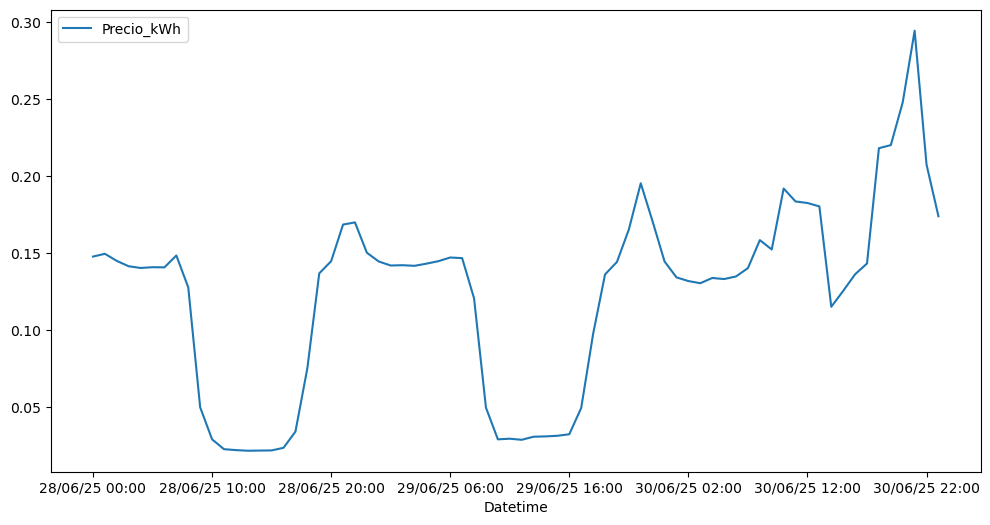
\includegraphics[width=\textwidth]{figuras/histoico.png}
\caption[Predicción mediante SARIMAX]{.}
\label{PrediccionSarimax}
\end{subfigure}
\begin{subfigure}[b]{0.3\textwidth}
\centering
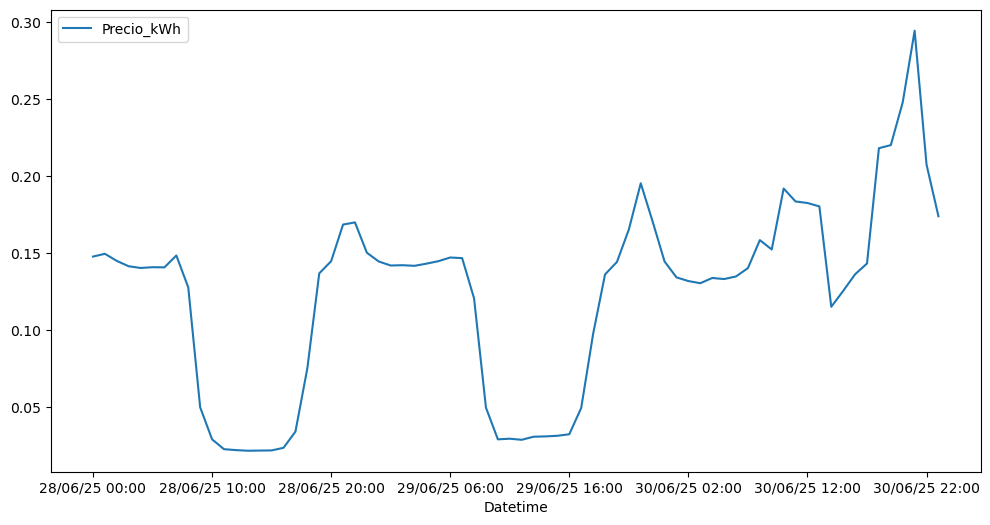
\includegraphics[width=\textwidth]{figuras/histoico.png}
\caption[Predicción mediante XGBoost]{.}
\label{PrediccionXGBoost}
\end{subfigure}
\begin{subfigure}[b]{0.3\textwidth}
\centering
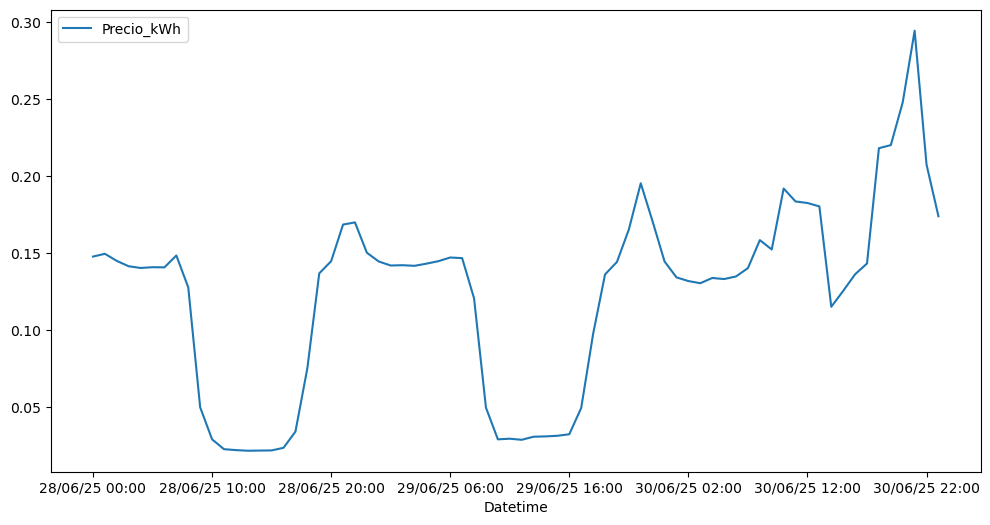
\includegraphics[width=\textwidth]{figuras/histoico.png}
\caption[Predicción mediante TFT]{.}
\label{PrediccionTFT}
\end{subfigure}
\caption{Predicciones para junio de 2025.}
\label{PrediccionesLuz}
\end{figure}
%
\subsection{Modelo físico}
%
%
Con el fin de explicar con algo de detalle cómo se modela un proceso de este tipo, voy a dar una introducción teórica del proceso, para traducirlo después a términos matemáticos. Como es comprensible, no se hicieron todos estos cálculos y las suposiciones y situaciones de la práctica ni requieren tanto tecnicismo ni lo requieren. Por esto, en la parte final de esta sección explicaré brevemente qué es lo que podría resultar útil de este planteamiento de cara a su implementación para una empresa.
%
%
%
\subsubsection{Situación simplificada: Primera aproximación} \label{PrimeraAproximacion}
%
%
%
Dado un metal conocido (X) de temperatura de fusión $T_f$, calor específico en los estados sólido y líquido, $c_{\text{sol}}$ y $c_{\text{liq}}$ respectivamente, entonces a la hora de conocer cuánta energía será necesaria tendremos que tener en cuenta:
\begin{itemize}
    \item[I] El metal X a una temperatura inicial $T_0$ debe ser calentado hasta la temperatura de fusión $T_f$, esto dependerá del \textit{calor específico} del material en el estado \textit{sólido}, que viene a ser el \textit{coste} energético para aumentar la temperatura del mismo.
    \item[II] Una vez alcanzado dicho objetivo el material cambia de estado de la materia requiriendo una nueva cantidad de calor dependiente del \textit{calor latente} del material, denominado como $L_{\text{s-l}}$.
    \item[III] Finalmente supondremos que seguiremos elevando la temperatura por lo que, de manera análoga al paso I, tendremos que tener en cuenta esta energía. Llamaremos a este límite $T_c$
\end{itemize}
Para realizar dichos cálculos, haremos uso de las fórmulas de calor para calor específico y transiciones de fase.
\begin{align}
    Q_{\text{pf}} &= m \cdot c_{\text{sol}} \cdot (T_f-T_0).\\
    Q_{\text{f}} &= m \cdot L.\\
    Q_{\text{e}} &= m \cdot c_{\text{liq}} \cdot (T_c-T_f).
\end{align}
De este modo, $Q = Q_{\text{pf}} + Q_{\text{f}} + Q_{\text{e}}$. Finalmente, deberíamos tener en cuenta que los hornos no son ideales y tenemos una cierta pérdida de energía. Este hecho, cuantificado por el rendimiento $\eta \in [0,1]$, provoca un aumento en el calor total necesario: $Q^{\text{tot}} = Q/\eta$.

\subsubsection{Situación general} \label{SituacionGeneral}
%
%
%
Nos situamos ahora ante el problema general, en el que partimos de temperaturas iniciales cercanas a la ambiente ($T_0 \simeq 25 \C$) mientras que llegamos a una temperatura final, $T_f$. En este caso tendremos que aplicar la formulación general:
\begin{equation}
    Q = m \cdot \int_{T_a}^{T_b} c(T)dT,
    \label{calor}
\end{equation}
donde $m$ es la masa del compuesto X y $c(T)$ es la función del calor específico con la temperatura. Para poder operar con esta expresión sería necesario consultar datos tabulados sobre el material y una vez obtenidos los datos de $c$ para distintas temperaturas, interpolamos para obtener una función con la que calcular, de manera aproximada, el calor en la \Cref{calor}.
De este modo llegaríamos a una situación similar a la descrita en la \Cref{PrimeraAproximacion}, obteniendo $Q^{\text{tot}}$. En ambos casos, como se va a tener desarrollo polinómico de $c(T)$, podemos calcular
\begin{align}
    Q & = m \cdot \int_{T_a}^{T_b} c(T)dT = m \cdot \int_{T_a}^{T_b} \Big[a_0+ a_1 T + \dots + a_nT^n \Big]dT = \\
    & = m \cdot \Big[a_0T+ \frac{a_1}{2} T^2 + \dots + \frac{a_n}{n+1} T^{n+1}\Big] \bigg|_{T_a}^{T_b} = m \cdot p(T_a, T_b),
\end{align}
donde sustituyendo obtenemos el valor deseado. Para el primer caso, tenemos que $T_a$ coincide con la temperatura \textit{ambiente} de la pieza mientras que $T_b$ con la de fusión del material X. Por otro lado, para la etapa final, la temperatura de fusión coincide con la inicial y la final que habíamos denominado $T_f$.
\subsubsection{Traducción matemática}
La situación anterior debe ser convenientemente planteada como restricciones, de cara a la resolución del problema de optimización con el que nos encontramos. Aunando lo descrito en la \Cref{SituacionGeneral} podemos escribir que el calor $Q$ necesario para la pieza X es:
\begin{equation}
    Q = Q_{\text{pf}} + Q_{\text{f}} + Q_{\text{e}} + Q' = m \cdot \Big( p_I + L + p_{III} \Big) + Q',
\end{equation}

Finalmente, debería considerarse el rendimiento $\eta$ del horno. Podríamos suponer que este valor es aproximadamente constante de manera que $\min{\eta f(x)} = \eta \min{f(x)}$, pudiendo prescindir de este valor. Si no fuera así deberíamos formularlo como una función e introducirlo en nuestro problema con sus correspondientes restricciones. Ya por último, se ha obtenido el calor $Q$ con unidad (J) \textit{julios}, mientras que habitualmente el coste eléctrico se da en \euro/kWh por lo que deberemos realizar la debida conversión. Esta, al igual que pasa con el rendimiento, influye en el valor numérico final pero no en el problema a optimizar.
%
%
\subsubsection{Implementación}
%
%
Como se ha mencionado, el trasfondo teórico de un proceso como este es, en muchos casos, innecesarios para dar una solución en el ámbito profesional, si bien es lo técnicamente correcto \footnote{Evidentemente, para llevarlo al grado más óptimo habría que introducir pérdidas de calor, más factores disipativos que puedan afectar al proceso, etc.}. Sin embargo, entender este planteamiento es importante debido a que la solución que se le otorga a una empresa está fundamenteada en ello.

Por lo general, no solo en este proyecto, sino también en la investigación realizada, lo más demandando en procesos de este tipo son las \textit{curvas de potencia} o respecto de otras magnitudes como el calor, temperatura... Del modelo planteado anteriormente podemos extraer ciertas conlusiones.

Es habitual que las empresas no tengan acceso a un histórico muy detallado del proceso, por lo que en ocasiones contamos con medidas escasas, sin embargo, podemos observar como la potencia ($P = Q/t$) crece de manera proporcional al calentamiento y depende directamente de la masa y las propiedades térmicas del material. Por ejemplo, una curva de potencia típica muestra cómo varía la demanda energética a lo largo del ciclo de fundición: inicialmente, la potencia requerida es mayor durante el calentamiento rápido, disminuyendo una vez alcanzada la temperatura de fusión y estabilizándose durante el mantenimiento térmico (una etapa muy común en fundiciones por ejemlpo para eliminar impurezas).

De igual modo, las curvas de temperatura permiten visualizar el perfil térmico de la pieza, identificando los puntos críticos del proceso (como el paso por la temperatura de fusión). Estas curvas son útiles para ajustar los hiperparámetros del horno, optimizar los tiempos de ciclo y prever posibles incidencias.
%
%
\subsection{Optimización de la superficie de enfriamiento}
%
%
El presente problema aborda la distribución de las piezas metálicas recién fundidas sobre la superficie de enfriamiento disponible en la nave. Cláramente, el objetivo es maximizar el número total de piezas que pueden colocarse simultáneamente. Esta superficie cuenta además con restricciones físicas relacionadas con la seguridad y operatividad del proceso, como márgenes laterales y pasillos interiores obligatorios de al menos 1.5 metros de ancho.

Cada pieza fundida es clasificada según su diametro y para su manipulación ha sido previamente colocada en una caja cuya dimensión se determina en función del tipo correspondiente. Estas cajas se disponen en planta sobre la superficie, sin posibilidad de apilarse. Una vez colocadas, no pueden solaparse ni invadir los pasillos o márgenes de seguridad. Es decir, deben respetarse las distancias mínimas entre ellas y con respecto a los bordes del área de enfriamiento. Esto impone restricciones geométricas estrictas sobre su posicionamiento.

El objetivo final es obtener una disposición óptima que maximice la cantidad total de piezas colocadas, permitiendo una planificación eficiente del enfriado. Dado el carácter discreto y combinatorio del problema, este puede abordarse mediante algoritmos de optimización específicos como métodos de empaquetado 2D, algoritmos genéticos o formulaciones de programación entera si se requiere una solución exacta.
%
%
